\documentclass[18pt, compress, aspectratio=169]{beamer}

% can be compiled by xelatex -shell-escape presentation.tex

\usetheme[usetitleprogressbar]{m}

\usepackage[utf8]{inputenc}
\usepackage[russian, english]{babel}
\usepackage{booktabs}
\usepackage[scale=2]{ccicons}
\usepackage{listings}
\usepackage{marvosym}
\usepackage{color}
\usepackage{xcolor}
\usepackage[document]{ragged2e}
\usepackage[export]{adjustbox}
\usepackage{fontawesome}
\usepackage{enumitem}
\usepackage{minted}
\usemintedstyle{tango}
%\usemintedstyle{monokai}

\usetikzlibrary{shapes,arrows,positioning}
\graphicspath{{images/}}
\newfontfamily{\FA}{FontAwesome}

\definecolor{check}{rgb}{0.1,2,0.3}
\definecolor{fail}{rgb}{2,0.1,0.1}
\definecolor{question}{rgb}{0.9,0.9,0.0}

\def\twitter{{\FA \faTwitter}}
\def\github{{\FA \faGithubSign}}
\def\email{{\FA \faEnvelope}}
\def\check{\textcolor{check}{\FA \faCheck}}
\def\fail{\textcolor{fail}{\FA \faRemove}}
\def\question{\textcolor{question}{\FA \faSearch}}

\renewcommand{\ttdefault}{pcr}
\newfontfamily{\ttfamily}{Fira Code}
\makeatletter
\newcommand\HUGE{\@setfontsize\Huge{38}{47}}
\makeatother

\definecolor{links}{HTML}{0099FF}
\hypersetup{colorlinks, linkcolor=, urlcolor=links}

\setbeamerfont{section title}{family=\Book, size=\Huge, shape=\normalfont}
\setbeamerfont{frametitle}{family=\Book, size=\large, shape=\normalfont}
\setbeamerfont{title}{family=\Book, size=\HUGE, shape=\normalfont}
\setbeamerfont{subtitle}{size=\Huge}

\title{FP в Python}
\subtitle{это проще, чем вы думали}
\date{\today}
\institute{}

\begin{document}
\fontsize{19pt}{20}\selectfont
\maketitle

\section{}

\begin{frame}{Контакты}
    \begin{itemize}[label={}]
        \item 
\includegraphics[scale=0.04]{mindojo_logo.png} Дмитрий Долгов, Mindojo
        \item {\github\ github.com/erthalion}
        \item {\twitter\ @erthalion}
        \item \email\ 9erthalion6 at gmail dot com
    \end{itemize}
\end{frame}

\begin{frame}[fragile]
    \frametitle{Для кого?}
    \begin{itemize}
        \item <+->
    \end{itemize}

    \vspace{-40pt}
    \begin{columns}[T,onlytextwidth]
    \column{0.5\textwidth}
    \begin{itemize}
        \item <+->
\includegraphics[width=7cm,height=4cm]{house1.jpeg}
    \end{itemize}

    \column{0.5\textwidth}
    \begin{itemize}
        \item <+->
\includegraphics[width=7cm,height=4cm]{house2.png}
    \end{itemize}
    \end{columns}
\end{frame}

\begin{frame}
    \frametitle{Причины?}
    \vspace{-25pt}
    \begin{figure}
        
\includegraphics[width=0.8\textwidth,center]{first_option.png}
    \end{figure}
\end{frame}

\begin{frame}
    \frametitle{Причины?}
    \vspace{-25pt}
    \begin{figure}
        
\includegraphics[width=0.8\textwidth,center]{second_option.png}
    \end{figure}
\end{frame}

\begin{frame}[fragile]
    \frametitle{Причины?}
    \begin{itemize}[label={\MVRightarrow}]
        \item FP - это парадигма, не привязанная к языку
        \item Python - мультипарадигменный язык,\\ позволяющий писать функционально
        \item Это позволяет увидеть преимущества FP в вашем коде уже завтра
    \end{itemize}
\end{frame}

\begin{frame}
    \frametitle{Плюсы и минусы}
    \vspace{-20pt}
    \begin{columns}[T,onlytextwidth]
    \column{0.5\textwidth}
        \begin{itemize}[label={\MVRightarrow}]
            \item <+->Разделение данных и логики \check
            \item <+->Модульность, легкое написание тестов \check
            \item <+->Распараллеливание кода \check
        \end{itemize}

    \column{0.45\textwidth}
        \begin{itemize}[label={\MVRightarrow}]
            \item <+->Сложно \fail
            \item <+->Страшно \fail
            \item <+->Разработчики? \fail
        \end{itemize}
    \end{columns}
\end{frame}

\begin{frame}[fragile]
    \frametitle{Кто?}
    \begin{itemize}[label={\MVRightarrow}]
        \item postgrest
        \item pandoc
        \item elm-compiler
        \item purescript
        \item aura (arch linux package manager)
    \end{itemize}
\end{frame}

\section{Краткое введение в FP}

\begin{frame}[fragile]
    \frametitle{Термины и определения}
    \begin{itemize}[label={\MVRightarrow}]
        \item Неизменяемость данных (immutability)
        \item Чистые функции и side effects
        \item Функции высшего порядка
        \item Монады (?)
        \item Abstract Data Type (ADT)
    \end{itemize}
\end{frame}

\begin{frame}
    \frametitle{Неизменяемость, персистентность}
    \vspace{-20pt}
    \begin{figure}
        
\includegraphics[width=1.0\textwidth,center]{Vault_Boy_text.png}
    \end{figure}
\end{frame}

\begin{frame}
    \frametitle{Чистые функции и side effects}
    \vspace{-25pt}
    \begin{figure}
        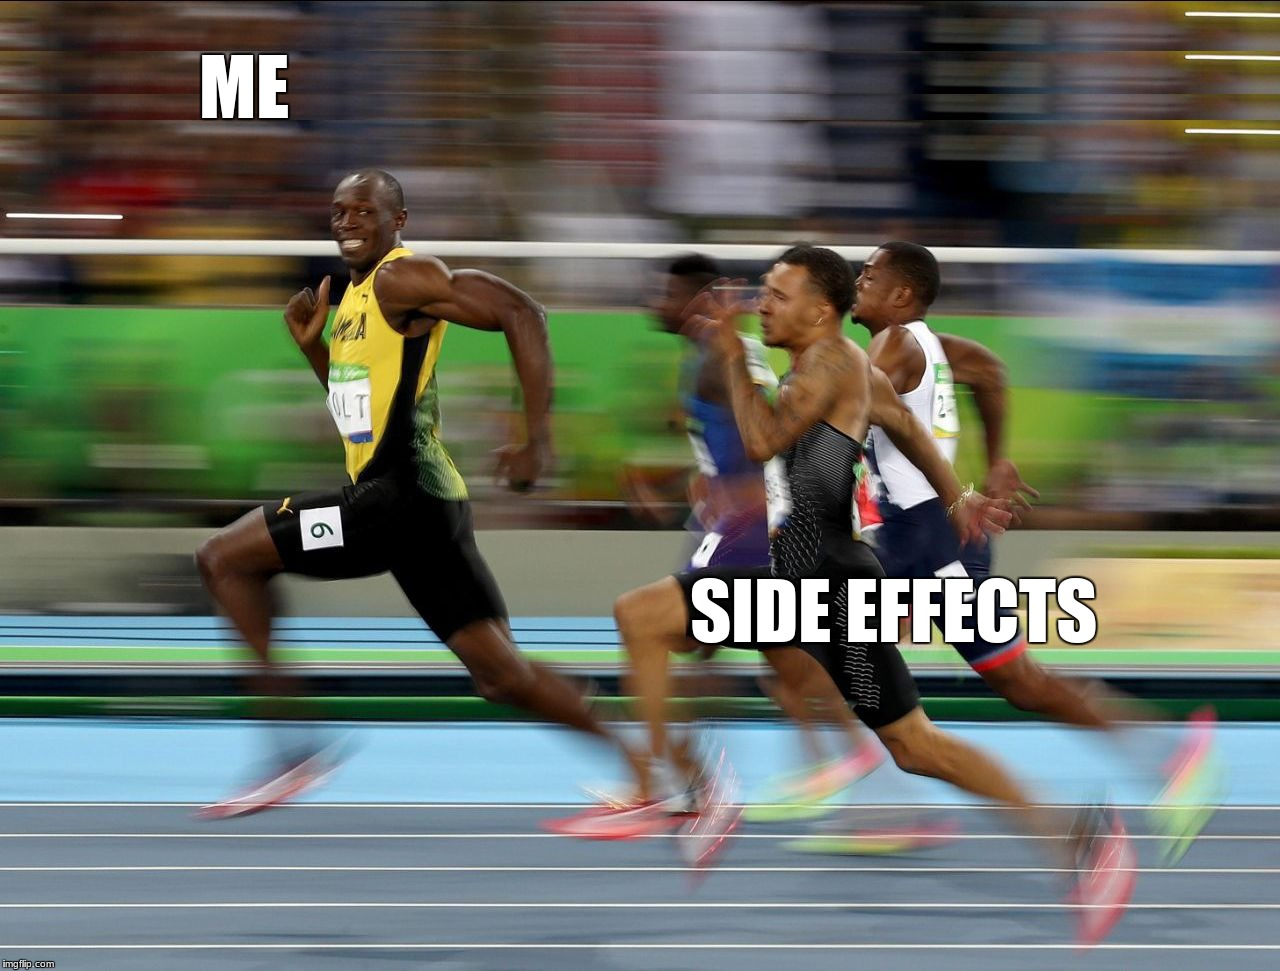
\includegraphics[width=0.7\textwidth,center]{side_effect.jpg}
    \end{figure}
\end{frame}

\begin{frame}
    \frametitle{Функции высшего порядка и композиция}
    \vspace{-25pt}
    \begin{figure}
        
\includegraphics[width=0.53\textwidth,center]{function_composition.jpg}
    \end{figure}
\end{frame}

\begin{frame}
    \frametitle{Монады, ADT}
    \vspace{-20pt}
    \begin{figure}
        
\includegraphics[width=0.5\textwidth,center]{squirells.png}
    \end{figure}
\end{frame}

\section{Возможности Python для FP}

\begin{frame}
    \frametitle{Что можно использовать?}
    \vspace{-25pt}
    \begin{itemize}[label={\MVRightarrow}]
        \item <+->Неизменяемые типы данных:
            \begin{itemize}
                \item string
                \item tuple/namedtuple
                \item fronzenset
            \end{itemize}
        \item <+->Функции высшего порядка
        \item <+->List comprehension
        \item <+->Generators
        \item <+->itertools
        \item <+->functools
    \end{itemize}
\end{frame}

\begin{frame}
    \frametitle{Что отсутствует?}
    \begin{overlayarea}{\textwidth}{.8\textheight}
    \begin{itemize}[label={\MVRightarrow}]
        \item <1->Хвостовая рекурсия \fail
        \item <2->Чистые функции \fail
        \item <3|only@3>Pattern matching \alt<3>{\fail}{\question}
        \item <4->Pattern matching \alt<3>{\fail}{\question}
        \item <5|only@5>Automatic currying \alt<5>{\fail}{\question}
        \item <6->Automatic currying \alt<5>{\fail}{\question}
        \item <7|only@7>Монады \alt<7>{\fail}{\question}
        \item <8->Монады \alt<7>{\fail}{\question}
        \item <9|only@9>ADT \alt<9>{\fail}{\question}
        \item <10->ADT \alt<9>{\fail}{\question}
    \end{itemize}
    \end{overlayarea}
\end{frame}

\begin{frame}
    \frametitle{Стратегии}
    \begin{itemize}[label={\MVRightarrow}]
        \item Использование <<чистого>> Python
        \item Собственные надстройки
        \item Сторонние библиотеки
    \end{itemize}
\end{frame}

\section{Примеры (py2)}

\setbeamercolor{background canvas}{bg=white}
\begin{frame}[fragile]
    \setbeamertemplate{section page}
    \frametitle{}
    \begin{center}
    \inputminted[
        fontsize=\large,
        %bgcolor=black,
    ]{python}{examples/immutable.py}
    \end{center}
\end{frame}

\begin{frame}[fragile]
    \setbeamertemplate{section page}
    \frametitle{}
    \begin{center}
    \inputminted[
        fontsize=\large,
    ]{python}{examples/list_comprehension.py}
    \inputminted[
        fontsize=\large,
    ]{haskell}{examples/list_comprehension.hs}
    \end{center}
\end{frame}

\begin{frame}[fragile]
    \setbeamertemplate{section page}
    \frametitle{}
    \begin{center}
    \inputminted[
        fontsize=\large,
    ]{python}{examples/generators.py}
    \end{center}
\end{frame}

\begin{frame}[fragile]
    \setbeamertemplate{section page}
    \frametitle{}
    \begin{center}
    \inputminted[
        fontsize=\large,
    ]{python}{examples/maybe_example.py}
    \end{center}
\end{frame}

\begin{frame}[fragile]
    \setbeamertemplate{section page}
    \frametitle{}
    \begin{center}
        \begin{figure}
            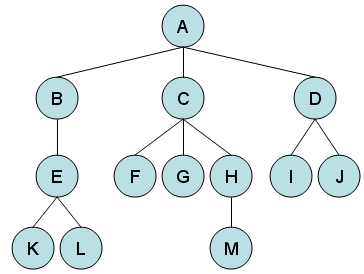
\includegraphics[width=0.5\textwidth,center]{tree.png}
        \end{figure}
    \end{center}
\end{frame}

\begin{frame}[fragile]
    \setbeamertemplate{section page}
    \frametitle{}
    \begin{center}
    \inputminted[
        fontsize=\large,
    ]{python}{examples/recursion_1.py}
    \end{center}
\end{frame}

\begin{frame}[fragile]
    \setbeamertemplate{section page}
    \frametitle{}
    \begin{center}
    \inputminted[
        fontsize=\large,
    ]{python}{examples/recursion_2.py}
    \end{center}
\end{frame}

\begin{frame}[fragile]
    \setbeamertemplate{section page}
    \frametitle{}
    \begin{center}
    \inputminted[
        fontsize=\large,
    ]{python}{examples/recursion_fp.py}
    \end{center}
\end{frame}

\begin{frame}[fragile]
    \setbeamertemplate{section page}
    \frametitle{}
    \begin{center}
    \inputminted[
        fontsize=\large,
    ]{python}{examples/curry_example1.py}
    \end{center}
\end{frame}

\begin{frame}[fragile]
    \setbeamertemplate{section page}
    \frametitle{}
    \begin{center}
    \inputminted[
        fontsize=\large,
    ]{python}{examples/curry_example2.py}
    \end{center}
\end{frame}

\begin{frame}[fragile]
    \setbeamertemplate{section page}
    \frametitle{}
    \begin{center}
    \inputminted[
        fontsize=\large,
    ]{python}{examples/example1.py}
    \end{center}
\end{frame}

\begin{frame}[fragile]
    \setbeamertemplate{section page}
    \frametitle{}
    \begin{center}
    \inputminted[
        fontsize=\large,
    ]{python}{examples/example2.py}
    \end{center}
\end{frame}

\begin{frame}[fragile]
    \setbeamertemplate{section page}
    \frametitle{}
    \begin{center}
    \inputminted[
        fontsize=\large,
    ]{python}{examples/example3.py}
    \end{center}
\end{frame}

\begin{frame}[fragile]
    \setbeamertemplate{section page}
    \frametitle{}
    \begin{center}
    \inputminted[
        fontsize=\large,
    ]{python}{examples/example4.py}
    \end{center}
\end{frame}
\note{http://programmers.stackexchange.com/questions/150837/maybe-monad-vs-exceptions}

\begin{frame}
    \vspace{7pt}
    \begin{figure}
        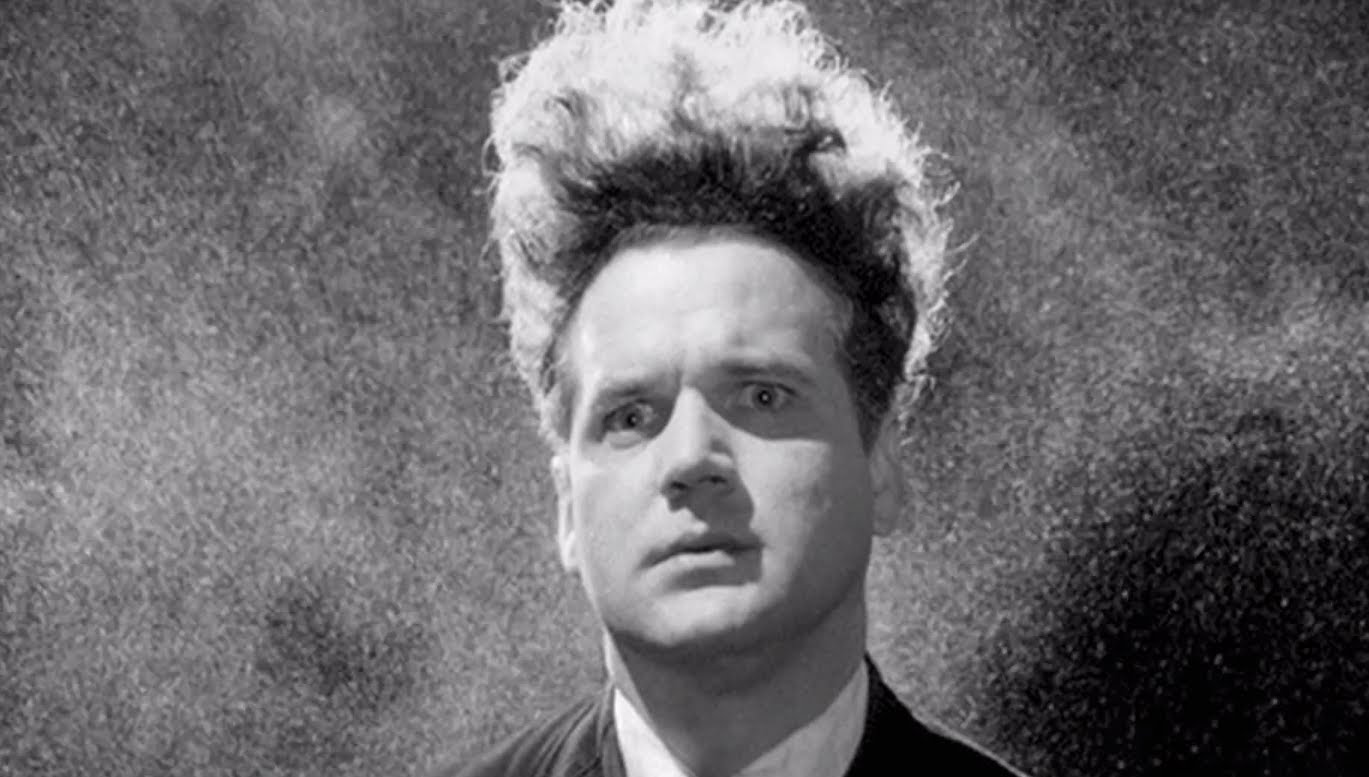
\includegraphics[width=1.0\textwidth,center]{mindblown.jpg}
    \end{figure}
\end{frame}

\setbeamercolor{background canvas}{bg=palette primary.bg}

\section{Библиотеки}

\fontsize{15pt}{16}\selectfont
\begin{frame}
    \frametitle{Список FP библиотек для Python}
    \vspace{-35pt}
    \begin{columns}[T,onlytextwidth]
        \column{0.5\textwidth}
        \begin{itemize}[label={\MVRightarrow}]
            \item PyFunctional
            \item toolz
            \item adt
            \item Coconat
            \item pyrsistent
            \item funcy
            \item effect
            \item hask
            \item fn.py
            \item PyMonad
        \end{itemize}

        \column{0.5\textwidth}
        \begin{itemize}[label={}]
            \item \href{github.com/EntilZha/PyFunctional}{EntilZha/PyFunctional}
            \item \href{github.com/pytoolz/toolz}{pytoolz/toolz}
            \item \href{github.com/llllllllll/adt}{llllllllll/adt}
            \item \href{github.com/evhub/coconut}{evhub/coconut}
            \item \href{github.com/Suor/funcy}{Suor/funcy}
            \item \href{github.com/tobgu/pyrsistent}{tobgu/pyrsistent}
            \item \href{github.com/python-effect/effect}{python-effect/effect}
            \item \href{github.com/billpmurphy/hask}{billpmurphy/hask}
            \item \href{github.com/kachayev/fn.py}{kachayev/fn.py}
            \item \href{github.com/fnl/pymonad}{fnl/pymonad}
        \end{itemize}

    \end{columns}
\end{frame}
\fontsize{19pt}{20}\selectfont

\begin{frame}
    \frametitle{Зачем?}
    \vspace{-25pt}
    \begin{itemize}[label={\MVRightarrow}]
        \item Функции на все случаи жизни
        \item Декоратор для каррирования
        \item Персистентные типы данных
        \item Синтаксис для функциональной композиции
        \item Декоратор для обхода хвостовой рекурсии
        \item Монады и ADT
    \end{itemize}
\end{frame}

\plain{Вопросы?}

\end{document}
